%%% Template originaly created by Karol Kozioł (mail@karol-koziol.net) and modified for ShareLaTeX use

\documentclass[a4paper,11pt]{article}

\usepackage[T1]{fontenc}
\usepackage[utf8]{inputenc}
\usepackage{graphicx}
\usepackage{xcolor}

\renewcommand\familydefault{\sfdefault}
\usepackage{tgheros}
\usepackage[defaultmono]{droidmono}

\usepackage{amsmath,amssymb,amsthm,textcomp}
\usepackage{enumerate}
\usepackage{multicol}
\usepackage{tikz}

\usepackage{geometry}
\geometry{left=25mm,right=25mm,%
bindingoffset=0mm, top=20mm,bottom=20mm}

\usepackage{float}

\linespread{1.3}

\newcommand{\linia}{\rule{\linewidth}{0.5pt}}

% custom theorems if needed
\newtheoremstyle{mytheor}
    {1ex}{1ex}{\normalfont}{0pt}{\scshape}{.}{1ex}
    {{\thmname{#1 }}{\thmnumber{#2}}{\thmnote{ (#3)}}}

\theoremstyle{mytheor}
\newtheorem{defi}{Definition}

% my own titles
\makeatletter
\renewcommand{\maketitle}{
\begin{center}
\vspace{2ex}
{\huge \textsc{\@title}}
\vspace{1ex}
\\
\linia\\
\@author \hfill \@date
\vspace{4ex}
\end{center}
}
\makeatother
%%%

% custom footers and headers
\usepackage{fancyhdr}
\pagestyle{fancy}
\lhead{}
\chead{}
\rhead{}
\lfoot{Assignment 2}
\cfoot{Approximation and randomized algorithms}
\rfoot{Page \thepage}
\renewcommand{\headrulewidth}{0pt}
\renewcommand{\footrulewidth}{0pt}
%

% code listing settings
\usepackage{listings}
\lstset{
    language=Python,
    basicstyle=\ttfamily\small,
    aboveskip={1.0\baselineskip},
    belowskip={1.0\baselineskip},
    columns=fixed,
    extendedchars=true,
    breaklines=true,
    tabsize=4,
    prebreak=\raisebox{0ex}[0ex][0ex]{\ensuremath{\hookleftarrow}},
    frame=lines,
    showtabs=false,
    showspaces=false,
    showstringspaces=false,
    keywordstyle=\color[rgb]{0.627,0.126,0.941},
    commentstyle=\color[rgb]{0.133,0.545,0.133},
    stringstyle=\color[rgb]{01,0,0},
    numbers=left,
    numberstyle=\small,
    stepnumber=1,
    numbersep=10pt,
    captionpos=t,
    escapeinside={\%*}{*)}
}

%%%----------%%%----------%%%----------%%%----------%%%

\begin{document}

\title{Assignment 2 \\\small{Sub-set Sum}}

\author{Matjaž Mav (63130148)}

\date{\today}

\maketitle

\section{DYN}
This approach has time complexity of $\mathcal{O}(n k)$ and space complexity of $\mathcal{O}(k)$. It is greatly effected by the size of array \textbf{\textit{A}} and/or targeted sum \textbf{\textit{k}}. If we introduce big numbers this problem becomes really hard for this approach. Example of such problem would be:

\begin{verbatim}
  5
  10000000
  2000000
  2000000
  2000000
  2000000
  2000000
\end{verbatim}

\section{EXH}
This approach has time and space complexity of $\mathcal{O}(2^n)$.
The worst case scenario is when the input is a long array \textbf{\textit{A}} of some relatively small numbers and some really big targeted sum \textbf{\textit{k}}. If the targeted sum \textbf{\textit{k}} is greater or equal then sum of the whole array \textbf{\textit{A}}, this approach will perform exhaustive search without any kind of pruning. Example of such problem would be:

\begin{verbatim}
  3000000
  6000000
  1
  2
  3
  1
  2
  3
  ...
  1
  2
  3
\end{verbatim}

\section{GREEDY}

This approach has time complexity of $\mathcal{O}(n \log{n})$ and space complexity of $\mathcal{O}(n)$. In the worst case this algorithm returns at most 2 times worse result. Example of such problem would be:

\begin{verbatim}
  3
  1000000
  500001
  500000
  500000
\end{verbatim}

In this case optimal result is $1000000$ but the algorithm would return $500001$. The result is almost 2 times worse then the optimal ($500001 \approx 1000000/2$).

\section{FPTAS}

First, we compared how the $\epsilon$ parameter effect the execution time of this algorithm on sorted lists. For this evaluation we have generated random inputs using code listed in the Listing 1 and then sort the elements in ascending and descending order. We observed (Figure \ref{img:eval-fptas-asc} and Figure \ref{img:eval-fptas-desc}) that on list sorted in descending order algorithm performs quicker and have much more stable execution time.

\begin{figure}[H]
  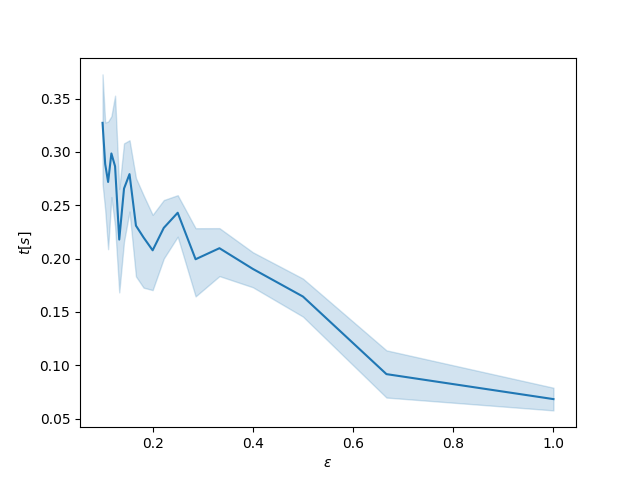
\includegraphics[width=.8\textwidth]{output/eval-fptas-asc}
  \centering
  \caption{Elements are sorted in ascending order. Execution time compared to the parameter $\epsilon$}
  \label{img:eval-fptas-asc}
\end{figure}

\begin{figure}[H]
  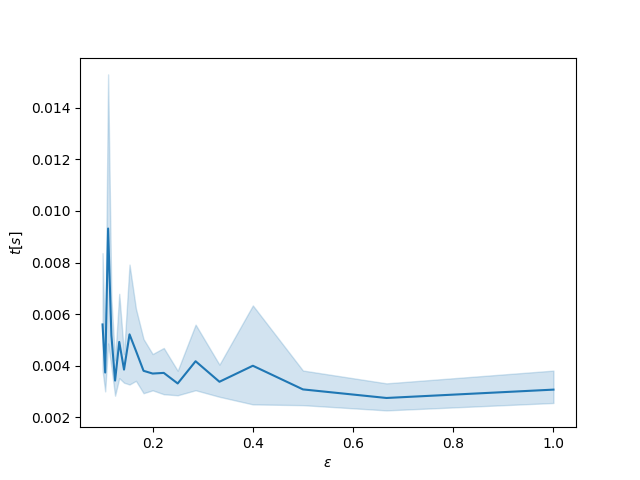
\includegraphics[width=.8\textwidth]{output/eval-fptas-desc}
  \centering
  \caption{Elements are sorted in descending order. Execution time compared to the parameter $\epsilon$}
  \label{img:eval-fptas-desc}
\end{figure}

Second, we upgrade our FPTAS implementation and first sorted elements in descending order. Then we generated exponential inputs using code listed in the Listing 2. From the Figure \ref{img:eval-fptas-hard} we can observe that FPTAS algorithm on the exponential generated inputs runs nearly 10 times slower on the random generated inputs.

\begin{figure}[H]
  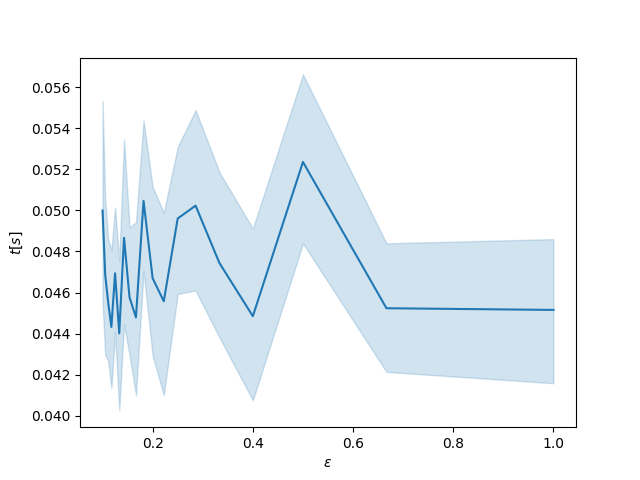
\includegraphics[width=.8\textwidth]{output/eval-fptas-hard}
  \centering
  \caption{Execution time compared to the parameter $\epsilon$}
  \label{img:eval-fptas-hard}
\end{figure}

\newpage
\lstinputlisting[
  language=Python,
  caption=Random problem generator,
  firstline=10,
  lastline=16
]{src/eval-fptas.py}

\lstinputlisting[
  language=Python,
  caption=Exponential problem generator,
  firstline=10,
  lastline=13
]{src/eval-fptas-hard.py}

\end{document}